\documentclass{beamer}
\usepackage{etex} % fixes new-dimension error
\usepackage{lmodern}
\usepackage[T1]{fontenc}
\usepackage[absolute,overlay]{textpos} % this is for textblock
\usepackage{tikz}
\usetikzlibrary{arrows.meta, calc, fit, tikzmark}
\usepackage{pgfplots}
\usepackage{multicol}
\usepackage{proof}
\usepackage{hyperref}
\usepackage{array} % m in tabularalso


%-------------- template --------------------------------------------------
\usetheme{metropolis}
\metroset{block=fill}
%\usetheme{Boadilla}

% Configuring the foot line
\setbeamertemplate{footline}
{
  \leavevmode%
  \hbox{%
  \begin{beamercolorbox}[wd=.4\paperwidth,ht=2.25ex,dp=1ex,center]{author in head/foot}%
    \usebeamerfont{author in head/foot}\insertshortauthor
  \end{beamercolorbox}%
  \begin{beamercolorbox}[wd=.5\paperwidth,ht=2.25ex,dp=1ex,center]{title in head/foot}%
    \usebeamerfont{title in head/foot}\insertsection
  \end{beamercolorbox}%
  \begin{beamercolorbox}[wd=.1\paperwidth,ht=2.25ex,dp=1ex,right]{date in head/foot}%
    \insertframenumber{} / \inserttotalframenumber\hspace*{2ex} 
  \end{beamercolorbox}}%
  \vskip0pt%
}
% No configuration symbols
\setbeamertemplate{navigation symbols}{}
%----------------------------------------------------------------------------

% context
\AtBeginSection[]
{
    \begin{frame}
        \frametitle{Table of Contents}
        \tableofcontents[currentsection]
    \end{frame}
}
\author[Renato Neves]{Renato Neves}
% logos of institutions
\titlegraphic{
  \begin{textblock*}{5cm}(6.7cm,7.57cm)
     
\includegraphics[scale=0.05525]{images/uminho.png}
  \end{textblock*}
  \begin{textblock*}{5cm}(9.4cm,7.57cm)
    
\includegraphics[scale=0.50]{images/haslab.pdf}
  \end{textblock*}
}
% No date
\date{}


%----------------------------------------------------------------------------
\usepackage{graphicx,amsmath}
\usepackage{stmaryrd} % cf. interleave
\usepackage{booktabs}
\usepackage{amscd}

\usepackage{alltt}
%------ using xy ------------------------------------------------------------
\usepackage[all]{xy}
%\def\larrow#1#2#3{\xymatrix{ #3 & #1 \ar[l] _-{#2} }}
\def\larrow#1#2#3{\xymatrix{ #3 & #1 \ar[l] _--{#2} }}
\def\rarrow#1#2#3{\xymatrix{ #1 \ar[r]^-{#2} & #3 }}
\def\arLaw#1#2#3#4#5{
\xymatrix{
        #1      \ar@/^1pc/[rr]^-{#4} &
        #5 &
        #2      \ar@/^1pc/[ll]^-{#3}
}}

\newcommand{\blue}[1]{\textcolor{blue}{#1}}
\begin{document}

\title{Semantics for (Hybrid) Programming}

\frame[plain]{\titlepage}

\section{Overview}

\begin{frame}{Last Lectures}
       
       Explored a simple language (\textsc{CCS}) and its semantics

       Used it to model and analyse \alert{communicating} systems

       Expanded our study to the \alert{timed} setting, via \textsc{UPPAAL}
       
       Used it to save us from zombies!

\end{frame}

\begin{frame}{Going Beyond the Timed Setting}
        \begin{minipage}[0.3\textheight]{\textwidth}
        \begin{columns}[c]
                \begin{column}{0.45\textwidth}
                \scalebox{0.6}{
                  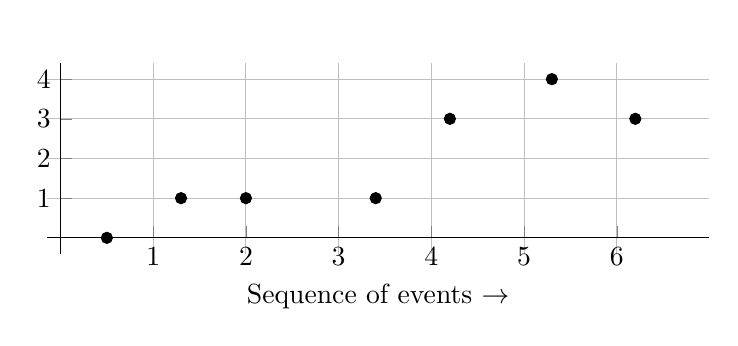
\begin{tikzpicture}
                   \begin{axis}[width=10cm, height=4cm, x axis line style={}, grid =
                     major, y axis line style={},
                     title={\textbf{}}, xlabel={\tikzmark{y1}\tikzmark{y2}Sequence
                     of events $\rightarrow$}, xtick =
                     {0,1,2,3,4,5,6}, xmax=7, axis lines*=center,
                     ytick={0,1,2,3,4,5,6},ylabel={},
                     xlabel near ticks, ylabel near ticks] \addplot [color=black,
                             only marks, domain = 0:5 ] 
                             coordinates {(0.5,0) (1.3,1) (2,1) (3.4,1) 
                             (4.2,3) (5.3,4) (6.2,3)};
                   \end{axis}
                  \end{tikzpicture}} 
                \end{column}
                \begin{column}{0.1\textwidth} 
                        \hspace{0.5cm} \textbf{+}                
                \end{column}
                \begin{column}{0.50\textwidth} 
                \scalebox{0.6}{ 
                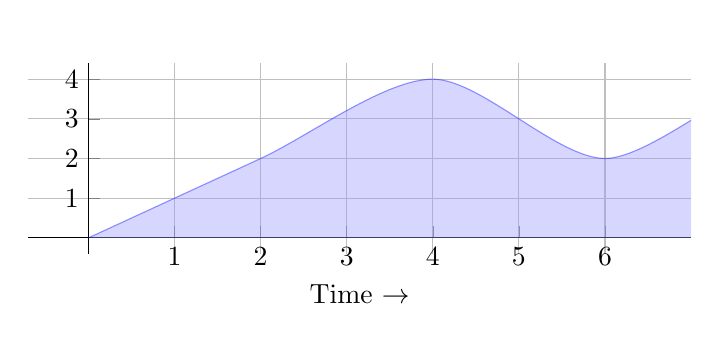
\begin{tikzpicture}
                \begin{axis}[width=10cm, height=4cm, x axis line style={}, grid =
                    major, y axis line style={},
                     title={\textbf{}}, xlabel={\tikzmark{x1}\tikzmark{x2}Time $\rightarrow$}				, xtick = {0,1,2,3,4,5,6} , xmax=7, axis lines*=center,
                     ytick={0,1,2,3,4,5,6}, ylabel={},
                     xlabel near ticks, ylabel near ticks] \addplot [color=blue, smooth,
                     domain = 0:5, fill = blue!40!white, opacity=0.4 ] coordinates {
                     (0,0) (2,2) (4,4) (6,2) (8,4) (8,0)};
                \end{axis}
                \end{tikzpicture}}
                \end{column}
        \end{columns}
        \end{minipage}

        \vspace{1.5cm}
        \begin{center}
                Computational devices now interact with \alert{arbitrary}
                physical processes (and not just time)
        \end{center}

        \begin{tikzpicture}[overlay,remember picture,
box/.style = {rounded corners},
pin edge={-Stealth,thick, red}]
\coordinate (x1) at ($({pic cs:x1})+(-4ex, 1.5ex)$);
\coordinate (x2) at ($({pic cs:x2})+(-5ex,-0.5ex)$);
\node[semitransparent,
     fit=(x1) (x2),
     pin=below:\tiny{Described via differential equations}]  {};
\end{tikzpicture} \begin{tikzpicture}[overlay,remember picture, box/.style
= {rounded corners}, pin edge={-Stealth,thick, red}] \coordinate (y1) at
     ($({pic cs:y1})+(-0.5ex, 1.5ex)$); \coordinate (y2) at ($({pic
     cs:y2})+(-1.5ex,-0.5ex)$); \node[semitransparent, fit=(y1) (y2),
     pin=below:\tiny{Described via classical methods of computation}]
{};
\end{tikzpicture}


\end{frame}

\begin{frame}{Which Language?}
        This time we explore a simple \alert{imperative
        language}

        No concurrency, no communication, and no higher-order func.

        (languages with such features are still underdeveloped)

        Perhaps some of you would like to improve them :-)
\end{frame}

\begin{frame}{The Hybrid While-Language}
        Fix a stock of variables $X = \{ \mathtt{x_1}, \dots , \mathtt{x_n}
	\}$. Then we have,

	\vspace{0.7cm}
	\begin{block}{Linear Terms}
	$\mathtt{LTerm}(X) \ni \tikzmark{r1}\mathtt{r}\tikzmark{r2} \mid \mathtt{r \cdot t}
        \mid \mathtt{x}  \mid \mathtt{t + s }$
	\end{block}

	\vspace{0.7cm}
	\begin{block}{Atomic Programs}
	$\mathtt{At}(X) \ni \mathtt{x := t} \mid
	\mathtt{x'_1 = t_1, \dots, x'_n = t_n \> \> \tikzmark{d1} \blue{for}\tikzmark{d2} 
	\> \> t }$
	\end{block}

	\vspace{0.7cm}
	\begin{block}{Hybrid Programs}
	$\mathtt{Prog}(X) \ni \mathtt{a} \mid
	\mathtt{p \> \blue{;} \> q} \mid
	\mathtt{\blue{if} \> b \> \blue{then} \> p \> \blue{else} \> q} \mid
	\mathtt{\blue{while} \> b \> \blue{do} \> \{ \> p \> \}}$
	\end{block}

	\begin{tikzpicture}[overlay,remember picture,
	box/.style = {rounded corners},
	pin edge={-Stealth,thick, red}]
	\coordinate (r1) at ($({pic cs:r1})+(-0.2ex, 1.5ex)$);
	\coordinate (r2) at ($({pic cs:r2})+(0.2ex,-0.5ex)$);
	\node[semitransparent,
	     fit=(r1) (r2),
	     pin=below:\tiny{real number}]  {};
	\end{tikzpicture}

	\begin{tikzpicture}[overlay,remember picture,
	box/.style = {rounded corners},
	pin edge={-Stealth,thick, red}]
	\coordinate (d1) at ($({pic cs:d1})+(-0.2ex, 1.5ex)$);
	\coordinate (d2) at ($({pic cs:d2})+(0.2ex,-0.5ex)$);
	\node[semitransparent,
	     fit=(d1) (d2),
	     pin=below:\tiny{"run" the system of differential 
	     equations for $\mathtt{t}$ seconds}]  {};
	\end{tikzpicture}

\end{frame}

\begin{frame}{Overview}

        First we tackle a \alert{while-language} without 
        differential equations and its semantics

        Then we move to the hybrid case 
        and see how the corresponding semantics helps the engineer to
        analyse
        hybrid programs

        Throughout this journey, we will:
        \begin{itemize}
                \item write implementations in \textsc{Haskell}
                \item do analyses in \textsc{Lince}
        \end{itemize}
\end{frame}

\section{Semantics for Linear Terms}

\begin{frame}{A Language of Linear Terms and its Semantics}

        \begin{block}{Linear Terms}
	$\mathtt{LTerm}(X) \ni \mathtt{r} \mid \mathtt{r \cdot t}
        \mid \mathtt{x}  \mid \mathtt{t + s }$
	\end{block}

        Let $\sigma : X \to \mathbb{R}$ be an \alert{environment}, i.e. a
        memory on which the program performs computations

        The expression $\langle \mathtt{t},\sigma \rangle \Downarrow
        \mathtt{r}$ tells that the linear expression $\mathtt{t}$ outputs
        $\mathtt{r}$ if the current memory is $\sigma$

        \[
                \infer[(\text{var})]{\langle \mathtt{x}, \sigma \rangle 
                \Downarrow \sigma(\mathtt{x})}{} \qquad \qquad
                \infer[(\text{con})]{\langle \mathtt{r}, \sigma \rangle 
                \Downarrow \mathtt{r}}{}
        \] \vspace{0.1cm}        
        \[        
                \infer[(\text{scl})]{  
                        \langle \mathtt{s} \cdot \mathtt{t}, \sigma \rangle \Downarrow 
                        \mathtt{s \cdot r}
                        }{
                        \langle \mathtt{t}, \sigma \rangle \Downarrow \mathtt{r}
                } \qquad \qquad
                \infer[(\text{add})]{  
                        \langle \mathtt{t_1} + \mathtt{t_2}, \sigma \rangle \Downarrow 
                        \mathtt{r_1 + r_2}
                        }{
                        \langle \mathtt{t_1}, \sigma \rangle \Downarrow \mathtt{r_1} \qquad
                        \langle \mathtt{t_2}, \sigma \rangle \Downarrow \mathtt{r_2}
                }
        \]
\end{frame}        

\begin{frame}{The Semantics at Work}
        The linear term $\mathtt{x + 2 \cdot y}$ corresponds to the tree 
        \[
                \xymatrix@C=10pt@R=10pt{
                        & (+) \ar[dl] \ar[dr]  & \\
                        \mathtt{x} & & \mathtt{(2\ \cdot)} \ar[d] \\
                        & & \mathtt{y} 
                }
        \]

        Consider an environment $\sigma$ such that $\sigma(\mathtt{x}) = 3$ and 
        $\sigma(\mathtt{y}) = 4$. We can then build the following derivation tree: 
        \[
                \infer{\langle \mathtt{ x + 2 \cdot y}, \sigma \rangle \Downarrow 
                \mathtt{11} }{
                        \langle \mathtt{x}, \sigma \rangle \Downarrow \mathtt{3} 
                        \qquad \qquad
                        \infer{\langle \mathtt{2 \cdot y}, \sigma \rangle \Downarrow 8}{
                        \langle \mathtt{y}, \sigma \rangle \Downarrow 4}
                }
        \]
\end{frame}

\begin{frame}{Exercises}
        \begin{itemize}
                \item $\langle \mathtt{2 \cdot x + 2 \cdot y}, \sigma \rangle \Downarrow$ ? 
                \item $\langle \mathtt{3 \cdot (2 \cdot x) + 2 \cdot (y + z)}, 
                        \sigma \rangle \Downarrow$ ? 
        \end{itemize}

        \pause
        \vfill
        Boring computations? If so why not implement the semantics in \textsc{Haskell}?
\end{frame}

\begin{frame}{Equivalence of Linear Terms}
        The previous semantics yields the following notion of 
        \alert{equivalence}: $\mathtt{t} \sim \mathtt{s}$ if for all
        environments $\sigma$
        \begin{flalign*}
                \langle \mathtt{t}, \sigma \rangle \Downarrow \mathtt{r} 
                \text{ iff } \langle \mathtt{s}, \sigma \rangle \Downarrow \mathtt{r}
        \end{flalign*}

        Examples of equivalent terms:
        \begin{itemize}
                \item $\mathtt{r \cdot (x + y)} \sim \mathtt{r \cdot x + r \cdot y}$
                \item $\mathtt{0 \cdot x} \sim \mathtt{0}$
                \item $\mathtt{(r \cdot s) \cdot x} \sim \mathtt{r \cdot (s \cdot x)}$ ?
        \end{itemize}
\end{frame}

\section{Semantics for Boolean Terms}

\begin{frame}{A Language of Boolean Terms and its Semantics}

        \begin{block}{Boolean Terms}
        $\mathtt{BTerm}(X) \ni \mathtt{t_1 \leq t_2} \mid \mathtt{b \wedge c}
        \mid \mathtt{\neg b}$
	\end{block}

        \pause
        The expression $\langle \mathtt{b},\sigma \rangle \Downarrow
        \mathtt{v}$ says that the Boolean term $\mathtt{b}$ outputs
        $\mathtt{v}$ if the current memory is $\sigma$

        \[
                \infer[(\text{leq})]
                { 
                        \langle \mathtt{t_1 \leq t_2}, \sigma \rangle \Downarrow \mathtt{tt} 
                }
                {
                        \langle \mathtt{t_1}, \sigma \rangle \Downarrow \mathtt{r_1} \qquad
                        \langle \mathtt{t_2}, \sigma \rangle \Downarrow \mathtt{r_2}
                        \qquad \mathtt{r_1 \leq r_2}
                } 
        \] 
        \[
                \infer[(\text{gtr})]
                { 
                        \langle \mathtt{t_1 \leq t_2}, \sigma \rangle \Downarrow \mathtt{ff} 
                }
                {
                        \langle \mathtt{t_1}, \sigma \rangle \Downarrow \mathtt{r_1} \qquad
                        \langle \mathtt{t_2}, \sigma \rangle \Downarrow \mathtt{r_2}
                        \qquad \mathtt{r_1 \not \leq r_2}
                }
        \]
        \[        
                \infer[(\text{not})]{  
                        \langle \mathtt{\neg \mathtt{b}}, \sigma \rangle \Downarrow 
                        \mathtt{\neg v}
                        }{
                        \langle \mathtt{b}, \sigma \rangle \Downarrow \mathtt{v}
                } \qquad \qquad
                \infer[(\text{and})]{  
                        \langle \mathtt{b_1} \wedge \mathtt{b_2}, \sigma \rangle \Downarrow 
                        \mathtt{v_1 \wedge v_2}
                        }{
                        \langle \mathtt{b_1}, \sigma \rangle \Downarrow \mathtt{v_1} \qquad
                        \langle \mathtt{b_2}, \sigma \rangle \Downarrow \mathtt{v_2}
                }
        \]
\end{frame}        

\section{Semantics for While Programs}

\begin{frame}{A While-language and its Semantics}
	\begin{block}{While-Programs}
	        $\mathtt{Prog}(X) \ni \mathtt{x := t} \mid
	        \mathtt{p \> \blue{;} \> q} \mid
	        \mathtt{\blue{if} \> b \> \blue{then} \> p \> \blue{else} \> q} \mid
	        \mathtt{\blue{while} \> b \> \blue{do} \> \{ \> p \> \}}$
        \end{block} \vspace{-0.4cm}
        \[
                \infer[(\text{asg})]{
                        \langle \mathtt{x := t}, \sigma \rangle \Downarrow 
                        \sigma[\mathtt{r} / \mathtt{x}]
                }{
                       \langle \mathtt{t}, \sigma \rangle \Downarrow \mathtt{r}
                } \hspace{1cm}
                \infer[(\text{seq})]{
                        \langle \mathtt{p \> \blue{;} \> q}, \sigma \rangle \Downarrow \sigma''
                }{
                        \langle \mathtt{p}, \sigma \rangle \Downarrow \sigma' \qquad
                        \langle \mathtt{q}, \sigma' \rangle \Downarrow \sigma'' 
                }
        \]\vspace{0.001cm}
        \[\hspace{-0.6cm}
                \infer[(\text{if1})]{
                        \langle \mathtt{\blue{if} \> b \> \blue{then} \> \> p \> \blue{else} \> q}, 
                        \sigma \rangle \Downarrow \sigma'
                }{
                        \langle \mathtt{b}, \sigma \rangle \Downarrow \mathtt{tt} \qquad
                        \langle \mathtt{p}, \sigma \rangle \Downarrow \sigma'
                } \hspace{1cm} 
                \infer[(\text{if2})]{
                        \langle \mathtt{\blue{if} \> b \> \blue{then} \> \> p \> \blue{else} \> q}, 
                        \sigma \rangle \Downarrow \sigma'
                }{
                        \langle \mathtt{b}, \sigma \rangle \Downarrow \mathtt{ff} \qquad
                        \langle \mathtt{q}, \sigma \rangle \Downarrow \sigma'
                } 
        \]\vspace{0.001cm}
        \[
                \infer[(\text{wh1})]{
                        \langle \mathtt{\blue{while} \> b \> \blue{do} \> \{ \> p \> \}}, \sigma \rangle
                        \Downarrow \sigma''
                }{
                        \langle \mathtt{b}, \sigma \rangle \Downarrow \mathtt{tt} \qquad
                        \langle \mathtt{p}, \sigma \rangle \Downarrow \sigma' \qquad
                        \langle \mathtt{\blue{while} \> b \> \blue{do} \> \{ \> p \> \}}, \sigma'
                        \rangle \Downarrow \sigma'' 
                }
        \]\vspace{0.001cm}
        \[
                \infer[(\text{wh2})]{
                        \langle \mathtt{\blue{while} \> b \> \blue{do} \> \{ \> p \> \}}, \sigma \rangle
                        \Downarrow \sigma
                }{
                        \langle \mathtt{b}, \sigma \rangle \Downarrow \mathtt{ff}
                }
        \]
\end{frame}
\begin{frame}{The Semantics at Work}
        The program $\mathtt{x := x + 1 \> \blue{;} \> x := x + 2}$ corresponds to the tree 
        \[
                \xymatrix@C=10pt@R=10pt{
                        & (\> ; \>) \ar[dl] \ar[dr]  & \\
                        \mathtt{x := x + 1} & & \mathtt{x := x + 2} 
                }
        \]

        Consider the environment $\sigma = x \mapsto 3$. 
        We build the following derivation tree: 
        \[
                \infer{
                        \langle \mathtt{ x := x + 1 \> \blue{;} \> x := x + 2 }, \mathtt{x \mapsto 3}
                        \rangle \Downarrow \mathtt{x \mapsto 6}
                }{
                        \infer{
                                \langle \mathtt{x := x +1}, \mathtt{x \mapsto 3} \rangle 
                                \Downarrow \mathtt{x \mapsto 4}
                        }{
                                \langle \mathtt{x + 1}, \mathtt{x \mapsto 3} \rangle \Downarrow
                                \mathtt{4}
                        }\qquad \qquad                        
                        \infer{
                                \langle \mathtt{x := x + 2}, \mathtt{x \mapsto 4} \rangle 
                                \Downarrow \mathtt{x \mapsto 6}
                        }{
                                \langle \mathtt{x + 2}, \mathtt{x \mapsto 4} \rangle \Downarrow
                                \mathtt{6}
                        }
                }
        \]
\end{frame}

\begin{frame}{Exercise}
        \begin{itemize}
                \item $\mathtt{x := 0 \> \blue{;} \> y := 1 \> \blue{;} \> 
                                \blue{while} \> x \leq y \> \blue{do} \> \{ x : = x + y \> \blue{;} \>
                        y := y + 1 \}} \Downarrow\ ?$
        \end{itemize}
\end{frame}

\begin{frame}{Equivalence of While-Programs}
        The previous semantics yields the following notion of 
        \alert{equivalence}: $\mathtt{p} \sim \mathtt{q}$ if for all
        environments $\sigma$
        \begin{flalign*}
                \langle \mathtt{p}, \sigma \rangle \Downarrow \mathtt{\sigma'} 
                \text{ iff } \langle \mathtt{q}, \sigma \rangle \Downarrow \mathtt{\sigma'}
        \end{flalign*}

        Examples of equivalent terms:
        \begin{itemize}
                \item $\mathtt{x := x + 1 \> \blue{;} \> x := x + 2 } 
                        \sim \mathtt{x := x + 3}$
                \item $\mathtt{(p \> \blue{;} \> q) \> \blue{;} \> r} \sim 
                        \mathtt{p \> \blue{;} \> (q \> \blue{;} \> r)}$
        \end{itemize}
\end{frame}

\begin{frame}{Pause for Meditations}

        We have just built and implemented our first progr. language
        
        Note that we used its semantics to \alert{run} our programs and also to
        \alert{prove} properties about them

        Which features would you like to add to this language next? Probabilistic
        operations or perhaps concurrency?
        
        Next step: add \alert{differential operations}
\end{frame}
\section{Semantics for Hybrid-while Programs}
\begin{frame}{Preliminaries about Differential Equations}
        Consider a stock $\mathcal{X} = \{ \mathtt{x_1}, \dots, \mathtt{x_n} \}$ of
        variables

        Systems of differential equations $\mathtt{x'_1 = t_1, \dots, x'_n =
        t_n}$ always have unique \alert{solutions}
        \[
                \tikzmark{sol1} \phi \tikzmark{sol2}: 
                \mathbb{R}^n \times [0,\infty) \longrightarrow \mathbb{R}^n
        \]

        \vspace{1cm}
        \begin{example}[The Continuous Dynamics of a Vehicle]
                $\mathtt{p' = v, v' = a}$ which admits the solution 
                \[
                        \phi((x_0,v_0),t) = \left (x_0 + v_0 t + 
                        \textstyle{\frac{1}{2}}a t^2, v_0 + at \right )
                \]
        \end{example}

	\begin{tikzpicture}[overlay,remember picture,
	box/.style = {rounded corners},
	pin edge={-Stealth,thick, red}]
	\coordinate (sol1) at ($({pic cs:sol1})+(-0.2ex, 1.5ex)$);
	\coordinate (sol2) at ($({pic cs:sol2})+(0.2ex,-0.5ex)$);
	\node[semitransparent,
	     fit=(sol1) (sol2),
	     pin=below:\tiny{Systematically obtained via linear algebra tools}]  {};
	\end{tikzpicture}

\end{frame}

\begin{frame}{Conventions}

        We will often abbreviate a list $v_1,\dots,v_n$ simply to $\overline{v}$

        $\sigma[\overline{v}/\overline{x}]$ denotes the environment that maps
        each $x_i$ in $\overline{x}$ to $v_i$ in $\overline{v}$ and all other
        variables the same way as $\sigma$

        \begin{example}
                \[
                        \sigma[v_1,v_2/x_1,x_2](y) = \begin{cases}
                                v_1 & \text{ if } y = x_1 \\
                                v_2 & \text{ if } y = x_2 \\
                                \sigma(y) & \text{ otherwise }
                        \end{cases}
                \]
        \end{example}

        We will often treat an environment $\sigma : \{ \mathtt{x_1}, \dots, \mathtt{x_n} \}
        \to \mathbb{R}$ as a list $[\sigma(\mathtt{x_1}), \dots, \sigma(\mathtt{x_n})]$
\end{frame}

\begin{frame}{The Hybrid While-Language and \dots}
        Fix a stock of variables $X = \{ \mathtt{x_1}, \dots , \mathtt{x_n}
	\}$. Then we have,

	\vspace{0.7cm}
	\begin{block}{Linear Terms}
	$\mathtt{LTerm}(X) \ni \tikzmark{r1}\mathtt{r}\tikzmark{r2} \mid \mathtt{r \cdot t}
        \mid \mathtt{x}  \mid \mathtt{t + s }$
	\end{block}

	\vspace{0.7cm}
	\begin{block}{Atomic Programs}
	$\mathtt{At}(X) \ni \mathtt{x := t} \mid
	\mathtt{x'_1 = t_1, \dots, x'_n = t_n \> \> \tikzmark{d1} \blue{for}\tikzmark{d2} 
	\> \> t }$
	\end{block}

	\vspace{0.7cm}
	\begin{block}{Hybrid Programs}
	$\mathtt{Prog}(X) \ni \mathtt{a} \mid
	\mathtt{p \> \blue{;} \> q} \mid
	\mathtt{\blue{if} \> b \> \blue{then} \> p \> \blue{else} \> q} \mid
	\mathtt{\blue{while} \> b \> \blue{do} \> \{ \> p \> \}}$
	\end{block}

	\begin{tikzpicture}[overlay,remember picture,
	box/.style = {rounded corners},
	pin edge={-Stealth,thick, red}]
	\coordinate (r1) at ($({pic cs:r1})+(-0.2ex, 1.5ex)$);
	\coordinate (r2) at ($({pic cs:r2})+(0.2ex,-0.5ex)$);
	\node[semitransparent,
	     fit=(r1) (r2),
	     pin=below:\tiny{real number}]  {};
	\end{tikzpicture}

	\begin{tikzpicture}[overlay,remember picture,
	box/.style = {rounded corners},
	pin edge={-Stealth,thick, red}]
	\coordinate (d1) at ($({pic cs:d1})+(-0.2ex, 1.5ex)$);
	\coordinate (d2) at ($({pic cs:d2})+(0.2ex,-0.5ex)$);
	\node[semitransparent,
	     fit=(d1) (d2),
	     pin=below:\tiny{"run" the system of differential 
	     equations for $\mathtt{t}$ seconds}]  {};
	\end{tikzpicture}
\end{frame}

\begin{frame}{ \dots\ its semantics }
        The evaluation of programs is now \alert{time-dependent}
        \[
                \langle \mathtt{p}, \sigma, \alert{t} \rangle \Downarrow \sigma'
        \]
        \dots\ different time instants, different outputs

        \textsc{Lince} relies on such a semantics: evaluating
        $\langle \mathtt{p}, \sigma, t_i \rangle$ for a "big"
        sequence $t_1, \dots, t_k$ results in a trajectory, such as

        \begin{center}
                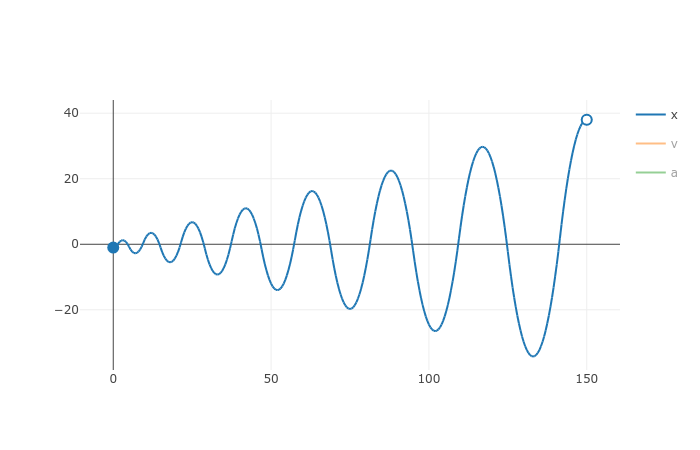
\includegraphics[scale=.22]{./images/traj.png}
        \end{center}
\end{frame}

\begin{frame}{The Semantic Rules pt. I}
        \[
                \infer{
                        \langle \overline{\mathtt{x}}' = \overline{\mathtt{t}} \> 
                        \blue{\mathtt{for}} \> \mathtt{s}, \sigma, t \rangle
                        \Downarrow \mathtt{stop}, \sigma[\phi(\sigma,t)/\overline{x}]
                }{
                        \langle \mathtt{s}, \sigma \rangle \Downarrow \mathtt{r}
                        \qquad t < \mathtt{r}
                }
        \]

        \[
                \infer{
                        \langle \overline{\mathtt{x}}' = \overline{\mathtt{t}} \> 
                        \blue{\mathtt{for}} \> \mathtt{s}, \sigma, t \rangle
                        \Downarrow \mathtt{skip}, \sigma[\phi(\sigma,t)/\overline{x}]
                }{
                        \langle \mathtt{s}, \sigma \rangle \Downarrow \mathtt{r}
                        \qquad t = \mathtt{r}
                }
        \]

        \[
                \infer[]{
                        \langle \mathtt{x := t}, \sigma,0 \rangle \Downarrow 
                        \sigma[\mathtt{r} / \mathtt{x}]
                }{
                       \langle \mathtt{t}, \sigma \rangle \Downarrow \mathtt{r}
                } \hspace{1cm}
                \infer[]{
                        \langle \mathtt{p \> \blue{;} \> q}, \sigma, t \rangle \Downarrow 
                        \mathtt{stop}, \sigma'
                }{
                        \langle \mathtt{p}, \sigma, t \rangle \Downarrow \mathtt{stop}, \sigma' 
                }
        \]

        \[
                \infer[]{
                        \langle \mathtt{p \> \blue{;} \> q}, \sigma, t + t' \rangle \Downarrow 
                        \mathtt{s}, \sigma''
                }{
                        \langle \mathtt{p}, \sigma, t \rangle \Downarrow \mathtt{skip}, \sigma' 
                        \qquad
                        \langle \mathtt{q}, \sigma, t' \rangle \Downarrow \mathtt{s}, \sigma''
                }
        \]
\end{frame}

\begin{frame}{Examples}
        \scriptsize
        \[
                \infer{
                        \langle (\mathtt{x' = 0} \> \mathtt{\blue{for}} \> 1) \>
                        \blue{\mathtt{;}} \> (\mathtt{x' = 1} \> \mathtt{\blue{for}} \> 1),
                        (\mathtt{x} \mapsto 2), \frac{1}{2} \rangle \Downarrow
                        \mathtt{stop}, (\mathtt{x} \mapsto 2) \tikzmark{no1} \tikzmark{no2}
                }{
                        \infer{ 
                                \langle \mathtt{x' = 0} \> \mathtt{\blue{for}} \> 1,
                                (\mathtt{x} \mapsto 2), \frac{1}{2} \rangle \Downarrow
                                \mathtt{stop}, (\mathtt{x} \mapsto 2) 
                        }{
                                \langle 1, (\mathtt{x} \mapsto 2) \rangle \Downarrow 1
                                \qquad
                                \frac{1}{2} < 1
                        }
                }
        \]         
        
        \vspace{0.8cm}
        \[      \hspace{-0.5cm}
                \infer{
                        \langle (\mathtt{x' = 0} \> \mathtt{\blue{for}} \> 1) \>
                        \blue{\mathtt{;}} \> (\mathtt{x' = 1} \> \mathtt{\blue{for}} \> 1),
                        (\mathtt{x} \mapsto 2), 1 + \frac{1}{2} \rangle \Downarrow
                        \mathtt{stop}, \tikzmark{so1} (\mathtt{x} \mapsto 2 + \frac{1}{2}) 
                        \tikzmark{so2}
                }{
                        \infer{ 
                                \langle \mathtt{x' = 0} \> \mathtt{\blue{for}} \> 1,
                                (\mathtt{x} \mapsto 2), 1 \rangle \Downarrow
                                \mathtt{skip}, (\mathtt{x} \mapsto 2) 
                        }{
                                \cdots                        
                        }
                        \qquad
                        \infer{
                                \langle \mathtt{x' = 1} \> \mathtt{\blue{for}} \> 1,
                                (\mathtt{x} \mapsto 2), \frac{1}{2} \rangle \Downarrow
                                \mathtt{stop}, (\mathtt{x} \mapsto 2 + \frac{1}{2})
                        }{
                                \cdots 
                        }
                }
        \]
        \begin{tikzpicture}[overlay,remember picture,
                box/.style = {rounded corners},
                pin edge={-Stealth,thick, red}]
                \coordinate (no1) at ($({pic cs:no1})+(-4ex, 1.5ex)$);
                \coordinate (no2) at ($({pic cs:no2})+(-5ex,-0.5ex)$);
                \node[semitransparent,
                        fit=(no1) (no2),
                        pin=below:\tiny{$= (\mathtt{x} \mapsto 2)
                        [\phi(2,\textstyle{\frac{1}{2}})/\mathtt{x}]$}]  {};
        \end{tikzpicture}
        \begin{tikzpicture}[overlay,remember picture,
                box/.style = {rounded corners},
                pin edge={-Stealth,thick, red}]
                \coordinate (so1) at ($({pic cs:so1})+(-4ex, 1.5ex)$);
                \coordinate (so2) at ($({pic cs:so2})+(-5ex,-0.5ex)$);
                \node[semitransparent,
                        fit=(so1) (so2),
                        pin=below:\tiny{$= (\mathtt{x} \mapsto 2)
                        [\phi(2,\textstyle{\frac{1}{2}})/\mathtt{x}]
                        = (\mathtt{x} \mapsto 2)
                        [2 + \textstyle{\frac{1}{2}}/\mathtt{x}] 
                        = x \mapsto 2 + \textstyle{\frac{1}{2}}$}]  {};
        \end{tikzpicture}
\end{frame}

\begin{frame}{Exercise}
        $\langle (\mathtt{x' = 1} \> \mathtt{\blue{for}} \> 1) \>
                        \blue{\mathtt{;}} \> (\mathtt{x' = -1} \> \mathtt{\blue{for}} \> 1),
                        (\mathtt{x} \mapsto 5), \frac{1}{2} \rangle \Downarrow\ ?$ 

                        \vspace{1cm}

        $\langle (\mathtt{x' = 1} \> \mathtt{\blue{for}} \> 1) \>
                        \blue{\mathtt{;}} \> (\mathtt{x' = -1} \> \mathtt{\blue{for}} \> 1),
                        (\mathtt{x} \mapsto 5), 2 \rangle \Downarrow\ ?$ 

\end{frame} 
\begin{frame}{The Semantic Rules pt. II}
        \[\hspace{-0.4cm}
                \infer[]{
                        \langle \mathtt{\blue{if} \> b \> \blue{then} \> \> p \> \blue{else} \> q}, 
                        \sigma, t \rangle \Downarrow \mathtt{s}, \sigma'
                }{
                        \langle \mathtt{b}, \sigma \rangle \Downarrow \mathtt{tt} \qquad
                        \langle \mathtt{p}, \sigma, t \rangle \Downarrow \mathtt{s}, \sigma'
                } \hspace{0.5cm} 
                \infer[]{
                        \langle \mathtt{\blue{if} \> b \> \blue{then} \> \> p \> \blue{else} \> q}, 
                        \sigma, t \rangle \Downarrow \mathtt{s}, \sigma'
                }{
                        \langle \mathtt{b}, \sigma \rangle \Downarrow \mathtt{ff} \qquad
                        \langle \mathtt{q}, \sigma, t \rangle \Downarrow \mathtt{s}, \sigma'
                } 
        \]

        \[
                \infer[]{
                        \langle \mathtt{\blue{while} \> b \> \blue{do} \> \{ \> p \> \}}, 
                        \sigma, t \rangle \Downarrow \mathtt{s}, \sigma'
                }{
                        \langle \mathtt{b}, \sigma \rangle \Downarrow \mathtt{tt} \qquad
                        \langle \mathtt{\mathtt{p} \> \blue{\mathtt{;}} \> 
                        \blue{while} \> b \> \blue{do} \> \{ \> p \> \}}, \sigma, t
                        \rangle \Downarrow \mathtt{s}, \sigma' 
                }
        \]\vspace{0.001cm}
        \[
                \infer[]{
                        \langle \mathtt{\blue{while} \> b \> \blue{do} \> \{ \> p \> \}}, \sigma 
                        , 0 \rangle \Downarrow \mathtt{skip},\sigma
                }{
                        \langle \mathtt{b}, \sigma \rangle\Downarrow  \mathtt{ff}
                }
        \]
\end{frame}

\begin{frame}{Equivalence of While-Programs}
        The previous semantics yields the following notion of 
        \alert{equivalence}: $\mathtt{p} \sim \mathtt{q}$ if for all
        environments $\sigma$ and time instants $t$,
        \begin{flalign*}
                \langle \mathtt{p}, \sigma, t \rangle \Downarrow \mathtt{s}, \mathtt{\sigma'} 
                \text{ iff } \langle \mathtt{q}, \sigma, t \rangle \Downarrow \mathtt{s}, 
                \mathtt{\sigma'}
        \end{flalign*}

        Examples of equivalent terms:
        \begin{itemize}
                \item $(\mathtt{x' = 1} \> \mathtt{\blue{for}} \> 1) \>
                        \blue{\mathtt{;}} \> (\mathtt{x' = 1} \> \mathtt{\blue{for}} \> 1)
                        \sim \mathtt{x' = 1} \> \mathtt{\blue{for}} \> 2$
                \item $\mathtt{(p \> \blue{;} \> q) \> \blue{;} \> r} \sim 
                        \mathtt{p \> \blue{;} \> (q \> \blue{;} \> r)}$
        \end{itemize}
\end{frame}
\section{A Zoo of Hybrid Programs}

\begin{frame}{A Zoo of Hybrid Programs}

        \begin{itemize}

                \item Traffic lights

                \item Cruise controller (speed regulation)

                \item Landing system

                \item \underline{Move a particle from A to B}

                \item \underline{Follow the leader}
        \end{itemize}

\end{frame} 
\begin{frame}{Analytical Testing and Following the Leader pt. I}
  \begin{minipage}[0.3\textheight]{\textwidth}
  \begin{columns}[c]
  \begin{column}{0.45\textwidth}
   \hspace{0.3cm}
   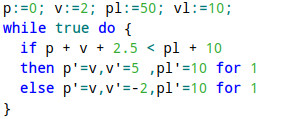
\includegraphics[scale=0.38]{./images/fl1.png}
  \end{column}
  \begin{column}{1\textwidth}
    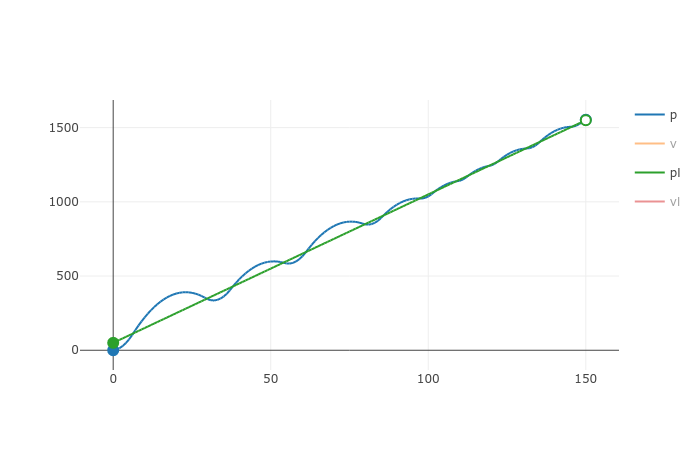
\includegraphics[scale=0.3]{./images/fl_plot.png}
  \end{column}
  \end{columns}
  \end{minipage}

  \pause
  Problem: Even if behind the leader in the next iteration, we might
  generate a velocity so high that we won't brake in time
\end{frame}

\begin{frame}{Analytical Testing and Following the Leader pt. II}
  \begin{minipage}[1\textheight]{\textwidth}
  \begin{columns}[c]
  \begin{column}{0.45\textwidth}
          \hspace{0.4cm} 
          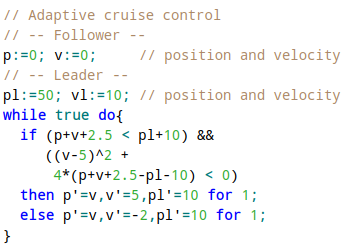
\includegraphics[scale=0.32]{./images/newcode.png}
  \end{column}
  \begin{column}{1\textwidth}
    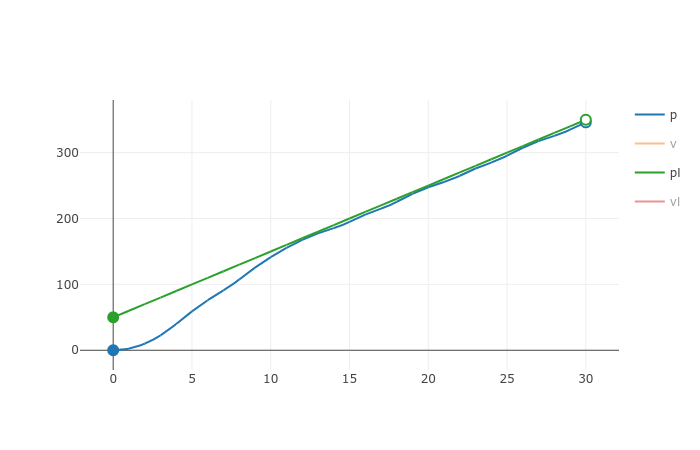
\includegraphics[scale=0.3]{./images/newplot.png}
  \end{column}
  \end{columns}
  \end{minipage}

  \pause
  \vspace{0.5cm}
  The conditional now arises from \alert{solving} the equation for $t$
  \[
        x_0 + v_0t + \frac{1}{2}(-2)t^2 = y_0 + 10t\ 
  \]
  No solutions, means no collisions!!
\end{frame}


\section{Examples of what not to do}

\begin{frame}{Checkpoint}
        We saw how to \alert{analyse} hybrid programs \alert{formally}

        We also visited a zoo of hybrid programs -- which improved our 
        ability to recognise them in the wild

        \pause
        What next?
\end{frame}


\begin{frame}{A Million-Dollar Question}
        How to simulate a differential statement that \alert{terminates
        as soon as} a certain \alert{event} occurs?  

        \[
                \mathtt{x}' = 1 \> \mathtt{\blue{until}} \> \mathtt{x = 2}
        \]

        \textbf{A:} No general solution for simulation with \alert{exact
        precision}; and even approximated simulation raises problems :-( 
        \[
                (\mathtt{x}' = 1 \> \mathtt{\blue{until}} \> \mathtt{x = 2}) \> \>
                \text{ collapses almost always to } \> \>
                (\mathtt{x}' = 1 \> \mathtt{\blue{for}} \> \mathtt{\infty})
        \]

        \vfill
        \pause
        For this lecture we take a (naive) approach:
        \[
                (\overline{\mathtt{x}}' = \overline{\mathtt{t}} \>
                \blue{\mathtt{until}}_\epsilon \> \mathtt{b}) \> \hat = \>
                \blue{\mathtt{while}} \> \neg \mathtt{b} \> \{ \overline{\mathtt{x}}' 
                = \overline{\mathtt{t}} \> \blue{\mathtt{for}} \> \epsilon \} 
        \]
        \end{frame}
\begin{frame}{(Another) Zoo of Hybrid Programs}
        \begin{itemize}
                \item Bouncing Ball
                \item Fireflies
        \end{itemize}

\end{frame}

\begin{frame}{Conclusions}
        Studied \alert{semantics} for (hybrid) prog. lang.

        Needed to interpret/analyse programs \alert{mathematically}

        Several case-studies left unexplored (e.g. movement in $n$-dimensions,
                orbital trajectories, trajectory correction)

        Several challenges left open (e.g. precise simulations, stability,
        uncertainty, recursion, concurrency, logical verification)
\end{frame}
\end{document}

